\graphicspath{{../../S02_Angles_particuliers/Images/}}

\themeG
\chapter{Angles particuliers}
\label{S02}


\textcolor{red}{\bf Connaissances :}
\begin{connaissances}
   \item Caractérisation angulaire du parallélisme : angles alternes-internes, angles correspondants.
\end{connaissances}

\vfill

\begin{debat}{Débat : angles et coordonnées géographiques}
   Tout point à la surface de la Terre est déterminé par ses coordonnées géographiques (la latitude et la longitude) et par son altitude (élévation par rapport au niveau de la mer). \par
   \begin{itemize}
      \item La {\bf latitude} d'un point sur la Terre est la mesure de l'angle que forment le plan de l'équateur et la demi-droite joignant le centre de la Terre à ce point.
      \item La {\bf longitude} d'un point est l'angle que fait le demi-plan passant par le méridien de ce point avec le plan du méridien de Greenwich.
   \end{itemize}
   Le collège Simone Veil se trouve à une latitude de 43,62 degrés Nord et 3,85 degrés Est.
   \tcblower
      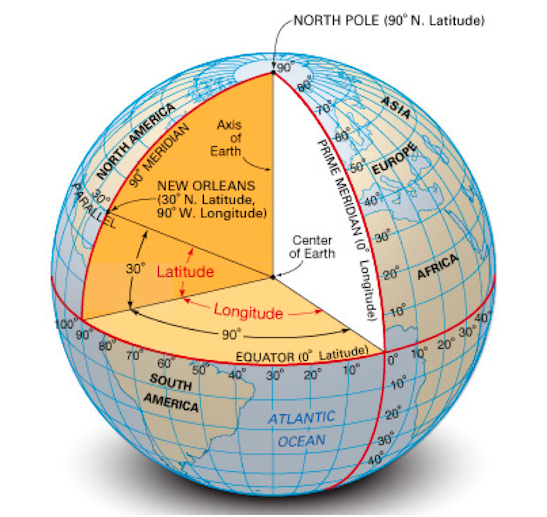
\includegraphics[width=5cm]{Longitude_latitude}
\end{debat}

\hfill {\gray Vidéo : \href{https://www.youtube.com/watch?v=lpYEuHeecko}{{\bf Les fondamentaux : latitude et longitude}, chaîne YouTube {\it La Classe d'Histoire}.}}


%%% Activité d'approche %%%
\begin{Maquette}[Cours]{Theme={Activité d'approche},Couleur={SteelBlue}}

   \AAtitre{Couples d'angles}
      {\it Objectifs : faire découvrir la notion d'angles-internes et d'angles correspondants.}

      \begin{AActivite}

         \begin{minipage}{10cm}
            \AApartie{Introduction}
               En utilisant les trois bandelettes modélisant trois droites $(d_1), (d_2)$ et $\Delta$ reliées entre elles par des attaches parisiennes, combien d'angles peut-on observer ? \pointilles
         \end{minipage}
         \hfill
         \begin{minipage}{6cm}
            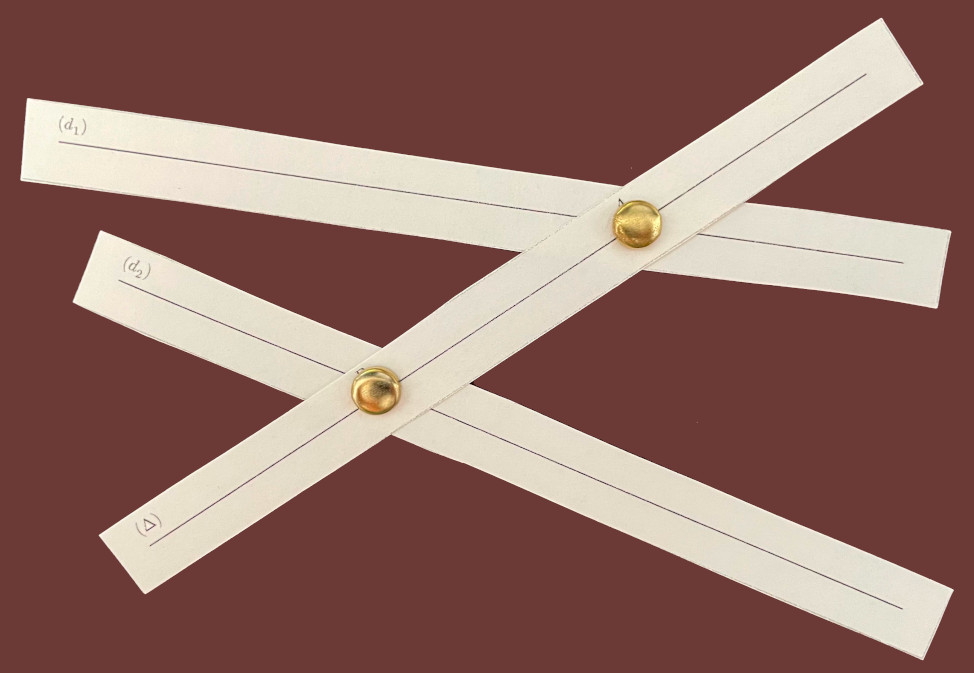
\includegraphics[width=6cm]{bandelettes}
         \end{minipage}

         \AApartie{Angles alternes-internes}
            \begin{enumerate}
               \item Prendre deux jetons, les placer sur deux angles vérifiant les conditions suivantes :
                  \begin{itemize}
                     \item les deux angles n'ont pas le même sommet ;
                     \item ils sont situés de part et d'autre de la droite $(\Delta)$ ;
                     \item ils sont situés \og entre \fg{} les droites $(d_1)$ et $(d_2)$.
                  \end{itemize}
                  Quelle est la mesure en degrés de chacun de ces deux angles ? \pointilles
               \item Combien y a-t-il de telles paires d'angles ? \pointilles \par
                  {\bf Les angles ainsi construits sont dit alternes-internes}.
               \item Placer les bandelettes de telle sorte que les droites $(d_1)$ et $(d_2)$ soient parallèles, repérer deux angles alternes-internes par deux jetons puis donner la mesure de chacun de ces deux angles. \pointilles
               \item En observant les résultats de la classe, quelle conjecture peut-on faire ? \par
                  \pointilles
            \end{enumerate}

         \AApartie{Angles correspondants}
            \begin{enumerate}[resume]
               \item Prendre deux jetons, les placer sur deux angles vérifiant les conditions suivantes :
                  \begin{itemize}
                     \item les deux angles n'ont pas le même sommet ;
                     \item ils sont situés du même côté que la droite $(\Delta)$ ;
                     \item l'un est situé \og entre \fg{} les droites $(d_1)$ et $(d_2)$, l'autre à l'extérieur.
                  \end{itemize}
                  Quelle est la mesure en degrés de chacun de ces deux angles ? \pointilles
               \item Combien y a-t-il de telles paires d'angles ? \pointilles \par
                  {\bf Les angles ainsi construits sont dit correspondants}.
               \item Placer les bandelettes de telle sorte que les droites $(d_1)$ et $(d_2)$ soient parallèles, repérer deux angles alternes-internes par deux jetons puis donner la mesure de chacun de ces deux angles. \pointilles
               \item En observant les résultats de la classe, quelle conjecture peut-on faire ? \par
                  \pointilles
            \end{enumerate}

      \end{AActivite}

\end{Maquette}


%%% Trace écrite %%%
\begin{Maquette}[Cours]{Theme={Trace écrite},Couleur={0.4[SteelBlue,Black]}}
   
   %%% 1
   \section{Mesure d'angles particuliers : rappels}

      \begin{minipage}{10.5cm}
         \begin{pspicture}(-5.5,-0.75)(5,2.5)
            \rput(0,-0.3){O}
            \rput(3.8,0){angle nul : 0°}
            \pswedge[fillstyle=solid,fillcolor=Crimson,linecolor=Crimson](0,0){1.5}{0}{90}
            \rput(2.5,1.3){\parbox{2.1cm}{\textcolor{Crimson}{angle aigu : \\ 0° < \pswedge[fillstyle=solid,fillcolor=Crimson,linecolor=Crimson](0.2,0){0.3}{0}{90} \qquad < 90°}}}
            \pswedge[fillstyle=solid,fillcolor=DodgerBlue,linecolor=DodgerBlue](0,0){1.5}{90}{180}
            \rput(-2.5,1.3){\parbox{2.5cm}{\textcolor{DodgerBlue}{angle obtus : \\ 90° < \pswedge[fillstyle=solid,fillcolor=DodgerBlue,linecolor=DodgerBlue](0.4,0){0.3}{90}{180} \quad\; < 180°}}}
            \rput(0,2.3){angle droit : 90°}
            \rput(-3.8,0){angle plat : 180°}
            \psline(-2.5,0)(2.5,0)
            \psline(0,2)
         \end{pspicture}   
      \end{minipage}
      \qquad
      \begin{minipage}{6cm}
         Dans cette configuration, la somme des deux angles mesure 180°, on dit que ces angles sont supplémentaires. \par
         \begin{pspicture}(0,-0.25)(6,1.5)
            \psline(0.5,0)(5.5,0)
            \psline(3,0)(1.8,1.2)
            \psarc[linecolor=Crimson](3,0){0.7}{135}{180}
            \rput(2,0.4){\textcolor{Crimson}{45°}}
            \psarc[linecolor=DodgerBlue](3,0){0.5}{0}{135}
            \rput(3.6,0.7){\textcolor{DodgerBlue}{135°}}
         \end{pspicture}
      \end{minipage}
   

   %%% 2
   \section{Angles alternes-internes et correspondants}
   
      \begin{minipage}{9cm}
         Lorsque deux droites sont coupées par une droite sécante $(\Delta)$, on obtient huit angles. \par
         {\it Dans la suite du cours, on se place dans cette configuration.}
      \end{minipage}
      \hfill 
      \begin{minipage}{6.5cm}
         \psset{unit=0.7}
         \begin{pspicture}(-1,-1)(6,3.5)
            \psline(0,1.5)(6,0.5)
            \psline(1,3)(6,3)
            \psline(1,0)(5,4)
            \psarc[linecolor=Crimson,doubleline=true](4,3){0.7}{0}{45}
            \rput(5,3.4){\textcolor{Crimson}{\small $A_2$}}
            \psarc[linecolor=DarkOrange,doubleline=true](4,3){0.7}{180}{225}
            \rput(3,2.5){\textcolor{DarkOrange}{\small $A_4$}}
            \psarc[linecolor=DodgerBlue](4,3){0.5}{45}{180}
            \rput(3.7,3.8){\textcolor{DodgerBlue}{\small $A_1$}}
            \psarc[linecolor=ForestGreen](4,3){0.5}{225}{0}
            \rput(4.35,2.25){\textcolor{ForestGreen}{\small $A_3$}}
            \psarc[linecolor=Crimson,doubleline=true](2.15,1.15){0.7}{-10}{45}
            \rput(3.2,1.4){\textcolor{Crimson}{\small $B_2$}}
            \psarc[linecolor=DarkOrange,doubleline=true](2.15,1.15){0.7}{170}{225}
            \rput(1.1,0.7){\textcolor{DarkOrange}{\small $B_4$}}
            \psarc[linecolor=DodgerBlue](2.15,1.15){0.5}{45}{170}
            \rput(1.8,1.9){\textcolor{DodgerBlue}{\small $B_1$}}
            \psarc[linecolor=ForestGreen](2.15,1.15){0.5}{225}{-10}
            \rput(2.4,0.3){\textcolor{ForestGreen}{\small $B_3$}}
            \rput(0.7,-0.3){$(\Delta)$}
            \rput(-0.5,1.5){$(d_1)$}
            \rput(0.5,3){$(d_2)$}
         \end{pspicture}
      \end{minipage}
      
      \begin{definition*}{}
         Deux angles sont {\bf alternes-internes} s'ils n'ont pas le même sommet, qu'ils sont situés de part et d'autre de la sécante $(\Delta)$ et qu'ils se situent \og entre \fg{} les droites $(d_1)$ et $(d_2)$.
      \end{definition*}
      
      \begin{exemple*}{}
         Sur la figure, il y a deux couples d'angles alternes-internes : $A_4$ et $B_2$ ; $A_3$ et $B_1$.
      \end{exemple*}
      
      \begin{definition*}{}
         Deux angles sont {\bf correspondants} s'ils n'ont pas le même sommet, qu'ils sont situés du même côté de la sécante $(\Delta)$, l'un entre les deux droites $(d_1)$ et $(d_2)$ et l'autre à l'extérieur.
      \end{definition*}
      
      \begin{exemple*}{}
         Sur la figure, il existe quatre couples d'angles correspondants :  $A_1$ et $B_1$ ; $A_2$ et $B_2$ ; $A_3$ et $B_3$ ; $A_4$ et $B_4$.
      \end{exemple*}
      
    
   %%%% 3
   \section{Et si les droites sont parallèles ?}
   
   \begin{propriete*}{}
      \begin{itemize}
         \item Si les deux droites $(d_1)$ et $(d_2)$ sont parallèles, alors les angles alternes-internes et les angles correspondants sont égaux deux à deux.
         \item Si deux angles alternes-internes ou deux angles correspondants sont égaux, alors les droites $(d_1)$ et $(d_2)$ sont parallèles.
      \end{itemize}
   \end{propriete*}
   
   \begin{exemple*}{}
      \begin{minipage}{6cm}
         \psset{unit=0.9}
         \begin{pspicture}(0,0.3)(6,3.2)
            \psline(1,1)(6,1)
            \psline(1,2.5)(6,2.5)
            \psline(2,0)(4,3)
            \rput(2.4,2.1){$\alpha =56°$}
            \rput(3.5,1.5){$\beta$}
            \rput(1.8,0.5){$\gamma$}
            \psarc[linecolor=Crimson,doubleline=true](3.67,2.5){0.6}{182}{234}
            \psarc[linecolor=DodgerBlue,doubleline=true](2.67,1){0.6}{2}{55}
            \psarc[linecolor=DarkOrange,doubleline=true](2.67,1){0.6}{182}{233}
            \rput(5.5,1.75){\parbox{1.5cm}{\small droites\\parallèles}}
         \end{pspicture}
      \end{minipage}
      \qquad
      \begin{minipage}{10cm}
         Mesures de $\beta$ et $\gamma$, sachant que les droites sont parallèles :
         \begin{itemize}
            \item $\alpha$ et $\beta$ sont des angles alternes-internes, ils ont donc même mesure. D'où : $\beta =\alpha =56°$.
            \item $\alpha$ et $\gamma$ sont des angles correspondants, ils ont donc même mesure. D'où : $\gamma =\alpha =56°$.
         \end{itemize}
      \end{minipage}
   \end{exemple*}

\end{Maquette}


%%% Exercices %%%
\begin{Maquette}[Fiche,CorrigeFin,Colonnes=2]{}

   \begin{multicols}{2}

      \begin{exercice} %1
         Au regard de la figure, que peut-on dire des angles :
         \begin{colenumerate}[3]%
            \item 1 et 5 ?
            \item 2 et 6 ?
            \item 4 et 6 ?
            \item 3 et 7 ?
            \item 3 et 5 ?
            \item 4 et 8 ?
         \end{colenumerate}
         {\psset{unit=0.7}
         \begin{pspicture}(-1.5,0)(6,4.5)
            \psline(0,1.5)(6,0.5)
            \psline(1,3)(6,3)
            \psline(1,0)(5,4)
            \psarc(4,3){0.7}{0}{45}
            \rput(5,3.4){2}
            \psarc(4,3){0.7}{180}{225}
            \rput(3,2.5){4}
            \psarc(4,3){0.5}{45}{180}
            \rput(3.7,3.8){1}
            \psarc(4,3){0.5}{225}{0}
            \rput(4.35,2.25){3}
            \psarc(2.15,1.15){0.7}{-10}{45}
            \rput(3.2,1.4){6}
            \psarc(2.15,1.15){0.7}{170}{225}
            \rput(1.1,0.7){8}
            \psarc(2.15,1.15){0.5}{45}{170}
            \rput(1.8,1.9){5}
            \psarc(2.15,1.15){0.5}{225}{-10}
            \rput(2.4,0.3){7}
         \end{pspicture}}
      \end{exercice}

      \begin{Solution}
         \begin{enumerate}
            \item Les angles 1 et 5 sont \cor{correspondants}.
            \item Les angles 2 et 6 sont \cor{correspondants}.
            \item Les angles 4 et 6 sont \cor{alternes-internes}.
            \item Les angles 3 et 7 sont \cor{correspondants}.
            \item Les angles 3 et 5 sont \cor{alternes-internes}.
            \item Les angles 4 et 8 sont \cor{correspondants}.
         \end{enumerate}
      \end{Solution}
      
      
      \begin{exercice} %2
         Dans la configuration suivante, citer :
         \begin{enumerate}
               \item la sécante ;
               \item deux angles correspondants ;
               \item deux angles alternes-internes.
         \end{enumerate}
         {\psset{unit=0.9}
         \begin{pspicture}(-3,-1.5)(3,1.2)
            \psline(-1.5,0)(2,0)
            \psline(-1,0.75)(2,-1.5)
            \psline(-1.5,-1)(2.5,-1)
            \rput(-1.75,0){$x$}
            \rput(-1.2,0.9){$y$}
            \rput(2.25,0){$t$}
            \rput(2.25,-1.6){$s$}
            \rput(2.75,-1){$u$}
            \rput(0.2,0.25){$O$}
            \rput(1.5,-0.75){$I$}
            \rput(-1.75,-1){$k$}
         \end{pspicture}}
      \end{exercice}

      \begin{Solution}
         \begin{enumerate}
            \item La sécante est \cor{la droite $(ys)$}.
            \item Il y a quatre couples d'angles correspondants : \par
               \cor{$\widehat{yOt}$ et $\widehat{OIu}$} ; \par
               \cor{$\widehat{yOx}$ et $\widehat{OIk}$} ; \par
               \cor{$\widehat{tOI}$ et $\widehat{uIs}$} ; \par
               \cor{$\widehat{xOI}$ et $\widehat{kIs}$}.
            \item Il y a deux couples d'angles alternes-internes : \par
               \cor{$\widehat{xOI}$ et $\widehat{OIu}$} \par
               \cor{$\widehat{tOI}$ et $\widehat{OIk}$}.
         \end{enumerate}
      \end{Solution}
      
      
      \begin{exercice}[Tout] %3
         Sur cette figure, les droites $(xy)$ et $(zt)$, ainsi que les droites $(su)$ et $(fg)$, sont parallèles. \par
         Compléter le tableau suivant lorsque c'est possible.
         \begin{center}
            \psset{xunit=1.8cm,yunit=0.8cm}
            \begin{pspicture}(-1.25,-2.2)(2.25,1.2)
               \psline(-1,0)(2,0)
               \psline(-1,-1)(2,-1)
               \psline(-1,1)(1,-2)
               \psline(0,1)(2,-2)
               \psline(0,-2)(1,1)
               \rput(-1.1,0){$x$}
               \rput(2.1,0){$y$}
               \rput(-1.1,-1){$z$}
               \rput(2.1,-1){$t$}
               \rput(-1.1,1.1){$s$}
               \rput(1.1,-2.1){$u$}
               \rput(-0.1,1.1){$f$}
               \rput(2.1,-2.1){$g$}      
               \rput(-0.1,-2.1){$h$}
               \rput(1.1,1.1){$i$}
               \rput(-0.3,0.25){$A$}
               \rput(0.85,0.2){$B$}
               \rput(0.3,-0.65){$C$}
               \rput(1.4,-0.65){$D$}
            \end{pspicture}
         \end{center}
         \begin{tabular}{|C{2.2}|*{4}{C{0.8}|}}
            \hline
            angle & $\widehat{yBg}$ & $\widehat{zCi}$ & $\widehat{fBi}$ & $\widehat{uCi}$ \\
            \hline
            alterne-interne & & & & \\
            \hline
            correspondant & & & & \\
            \hline
         \end{tabular}
      \end{exercice}

      \begin{Solution}
         On obtient le tableau suivant, par exemple : \par \smallskip
         {\hautab{2}
         \begin{tabular}{|C{1.8}|*{4}{C{0.85}|}}
            \hline
            angle & $\widehat{yBg}$ & $\widehat{zCi}$ & $\widehat{fBi}$ & $\widehat{uCi}$ \\
            \hline
            \footnotesize Angles alterne-interne & \textcolor{RoyalBlue}{$\widehat{zDf}$ $\widehat{BDC}$\dots} & \textcolor{RoyalBlue}{$\widehat{hBy}$ $\widehat{yBC}$\dots} & \textcolor{RoyalBlue}{$\varnothing$} & \textcolor{RoyalBlue}{$\widehat{fBh}$ $\widehat{CBf}$\dots} \\
            \hline
            \footnotesize Angles correspondant & \textcolor{RoyalBlue}{$\widehat{tDg}$ $\widehat{yAu}$\dots} & \textcolor{RoyalBlue}{$\widehat{xBi}$ $\widehat{iBA}$\dots} & \textcolor{RoyalBlue}{$\widehat{sCi}$ $\widehat{BCA}$\dots} & \textcolor{RoyalBlue}{$\widehat{gBi}$ $\widehat{iBD}$\dots} \\
            \hline
         \end{tabular}}
      \end{Solution}
      
      
      \begin{exercice} %4
         Batoul pense que l'une des deux paires de droites $(d_1)$ et $(d_2)$ est parallèle. A-t-elle raison ? Justifier \par
         {\psset{unit=0.8}
         \begin{pspicture}(0.2,-0.2)(4,2.5)
            \pstGeonode[PointSymbol=none,PointName=none](0,2.5){A}(4,0){B}(0,1){C}(3,2){D}(1,0){E}(4,1){F}
            \pstInterLL[PointName=none,PointSymbol=none]{A}{B}{C}{D}{H}
            \pstInterLL[PointName=none,PointSymbol=none]{A}{B}{E}{F}{I}
            \pstLineAB{A}{B}
            \pstLineAB{C}{D}
            \pstLineAB{E}{F}
            \pstMarkAngle{D}{H}{A}{119°}
            \pstMarkAngle{B}{I}{F}{61°}
            \rput(0.5,0.8){$(d_1)$}
            \rput(1.7,-0.2){$(d_2)$}
         \end{pspicture} 
         \begin{pspicture}(-1,-0.2)(3.3,3.2)
            \pstGeonode[PointSymbol=none,PointName=none](0,1.5){A}(3,1){B}(0,0){C}(1.5,3){D}(1.5,0){E}(2.5,2.5){F}
            \pstInterLL[PointName=none,PointSymbol=none]{A}{B}{C}{D}{H}
            \pstInterLL[PointName=none,PointSymbol=none]{A}{B}{E}{F}{I}
            \pstLineAB{A}{B}
            \pstLineAB{C}{D}
            \pstLineAB{E}{F}
            \pstMarkAngle{B}{H}{D}{59°}
            \pstMarkAngle{E}{I}{B}{111°}
            \rput(1,2.8){$(d_1)$}
            \rput(3,2.5){$(d_2)$}
         \end{pspicture}}
      \end{exercice}

      \begin{Solution}
         Oui, Batoul a raison : \par
         \begin{itemize}
            \item Première figure : l'angle supplémentaire à 119° de l'autre côté de $(d_1)$ vaut $180°-119° =61°$. \par
               On a deux angles correspondants de même mesure donc, \cor{les droites $(d_1)$ et $(d_2)$ sont parallèles}.
            \item Deuxième figure : l'angle supplémentaire à 111° de l'autre côté de $(d_2)$ vaut $180°-111° =69°$. \par
               On a deux angles alternes-internes de mesures différentes donc, \cor{$(d_1)$ et $(d_2)$ ne sont pas parallèles}.
         \end{itemize}
      \end{Solution}
      
      
      \begin{exercice} %5
         Dans la figure ci-dessous, on sait que les droites $(xy)$ et $(tz)$ sont parallèles et on connaît la mesure de deux angles. En utilisant les données de la figure :
         \begin{enumerate}
            \item Donner la mesure en degrés d'un maximum d'angles de la figure.
            \item En déduire la nature du triangle $IJK$?
         \end{enumerate}
         \begin{pspicture}(-2,-0.5)(4.8,3)
            \pstGeonode[PointSymbol=none,PosAngle={180,120,-120,0,180,0}](-1,0){z}(0,0){K}(2,0){J}(4,0){t}
            \pstRotation[PointSymbol=none,PosAngle=150,RotAngle=60]{K}{J}[I]
            \pstOIJGeonode[PointSymbol=none,PosAngle={180,0,60,120}](-1,1){x}{K}{J}{I}(1.5,1){y}(0,1.4){s}(-.4,1.4){r}
            \pstLineAB{x}{y}
            \pstLineAB{z}{t}
            \pstLineAB[nodesepA=-.9,nodesepB=-.5]{I}{K}
            \pstLineAB[nodesepA=-.9, nodesepB=-.5]{I}{J}
            \pstMarkAngle{t}{J}{r}{120°}
            \pstMarkAngle{y}{I}{s}{60°}
         \end{pspicture}
      \end{exercice}

      \begin{Solution}
         \begin{enumerate}
            \item $\bullet$ Les angles $\widehat{IJK}$ et $\widehat{IJt}$ sont supplémentaires \par
               donc, $\cor{\widehat{IJK}} =180°-120°° =\cor{60°}$. \par
               $\bullet$ Les angles $\widehat{JKI}$ et $\widehat{yIS}$ sont correspondants et $\widehat{yIS} =60°$ \par
               donc, \cor{$\widehat{JKI} =60°$}. \par
               $\bullet$ Les angles $\widehat{rIy}$ et $\widehat{IJt}$ sont correspondants et $\widehat{IJt} =120°$ \par
               donc, \cor{$\widehat{rIy} =120°$}. \par
               $\bullet$ Les angles $\widehat{yIJ}$ et $\widehat{rIy}$ sont supplémentaires \par
               donc, $\cor{\widehat{yIJ}} =180°-120°° =\cor{60°}$. \par
               $\bullet$ Les angles $\widehat{xIK}$ et $\widehat{sIy}$ sont opposés par le sommet \par
               donc, $\cor{\widehat{xIK}} =\widehat{sIy} =\cor{60°}$. Et enfin : \par
               $\cor{\widehat{KIJ}} =180° -\widehat{xIK}-\widehat{yIJ}$ \par
               $=180°-60°-60° =\cor{60°}$.
            \item Les trois angles du triangle sont égaux, donc \cor{le triangle $IJK$ est équilatéral}.
         \end{enumerate}
      \end{Solution}
      
      
      \begin{exercice}[Dur] %6
         Sur la figure ci-dessous :
         \begin{itemize}
            \item les droites $(ab), (cd)$ et $(ef)$ sont parallèles ;
            \item $R$ est un point de $(ab)$, $S$ un point de $(cd)$ et $T$ un point de $(ef)$ tels que $\widehat{bRS} =20°$ et $\widehat{RST} =57°$.
         \end{itemize}
         Calculer la mesure de l'angle $\widehat{STf}$. \par
         \begin{pspicture}(-0.5,0.2)(7,3.8)
            \pstGeonode[PointSymbol=none,PosAngle={90}](0,0.5){e}(2,0.5){T}(7,0.5){f}(0,2){c}(4,2){S}(7,2){d}(0,3){a}(2,3){R}(7,3){b}
            \pstLineAB{a}{b}
            \pstLineAB{c}{d}
            \pstLineAB{e}{f}
            \pstLineAB{R}{S}
            \pstLineAB{S}{T}
            \pstMarkAngle{S}{R}{b}{}
            \rput(3,2.8){20°}
            \pstMarkAngle[MarkAngleType=double]{R}{S}{T}{}
            \rput(3.2,1.8){57°}
            \pstMarkAngle{f}{T}{S}{?}
         \end{pspicture}
      \end{exercice}

      \begin{Solution}
         \begin{itemize}
            \item Les angles $\widehat{bRS}$ et $\widehat{RSc}$ sont alternes-internes et les droites $(ab)$ et $(cd)$ sont parallèles donc : $\widehat{RSc} =\widehat{bRS} =20°$.
            \item On décompose l'angle $\widehat{RST}$ : $\widehat{RST} =\widehat{RSc}+\widehat{cST}$ donc, $\widehat{cST} =\widehat{RST} -\widehat{RSc} =57°-20° =37°$.
            \item Les angles $\widehat{cST}$ et $\widehat{STf}$ sont alternes-internes et les droites $(cd)$ et $(ef)$ sont parallèles donc : $\widehat{STf} =\widehat{cST} =\blue 37°$.
         \end{itemize}
      \end{Solution}
      
      
      \begin{exercice}[Dur] %7
         Léon possède un champ en forme de quadrilatère $LEON$ dont les côtés $(LE)$ et $(ON)$ sont parallèles. Il prend la mesure de deux angles et se demande si son quadrilatère peut être un parallélogramme.
         \begin{enumerate}
            \item Écrire sur le schéma ci-dessous la mesure de tous les angles existants.
            \item Les droites $(LN)$ et $(EO)$ sont-elles parallèles ?
            \item Quelle est alors la nature du quadrilatère $LEON$ ?
         \end{enumerate}
         {\psset{unit=0.6}
         \begin{pspicture}(-1,0)(10,6)
            \pstGeonode[PointSymbol=none,PointName=none](0,1){a}(10,1){b}(0,4){c}(10,4){d}(0.33,0){f}(4,5.5){g}(6.33,0){h}(9,5){j}
            \pstLineAB{a}{b}
            \pstLineAB{c}{d}
            \pstLineAB{f}{g}
            \pstLineAB{h}{j}
            \pstInterLL[PosAngle=-45,PointSymbol=none]{a}{b}{f}{g}{N}
            \pstInterLL[PosAngle=-45,PointSymbol=none]{a}{b}{h}{j}{O}
            \pstInterLL[PosAngle=-45,PointSymbol=none]{c}{d}{f}{g}{L}
            \pstInterLL[PosAngle=-45,PointSymbol=none]{c}{d}{h}{j}{E}
            \pstMarkAngle{j}{E}{L}{121°}
            \pstMarkAngle{O}{N}{L}{49°}
         \end{pspicture}}
      \end{exercice}
      
      \begin{Solution}
         \begin{enumerate}
            \item Schéma du terrain de Léon : \par
               {\psset{unit=0.7}
               \begin{pspicture}(-0.5,-0.5)(10,6)
                  \pstGeonode[PointSymbol=none,PointName=none](0,1){a}(10,1){b}(0,4){c}(10,4){d}(0.33,0){f}(4.5,5.5){g}(6.33,0){h}(9,5){j}
                  \pstLineAB{a}{b}
                  \pstLineAB{c}{d}
                  \pstLineAB{f}{g}
                  \pstLineAB{h}{j}
                  \pstInterLL[PosAngle=-45,PointSymbol=none,PointName=none]{a}{b}{f}{g}{S}
                  \pstInterLL[PosAngle=-45,PointSymbol=none,PointName=none]{a}{b}{h}{j}{E}
                  \pstInterLL[PosAngle=-45,PointSymbol=none,PointName=none]{c}{d}{f}{g}{I}
                  \pstInterLL[PosAngle=-45,PointSymbol=none,PointName=none]{c}{d}{h}{j}{N}
                  \pstMarkAngle{j}{N}{I}{121°}
                  \pstMarkAngle{E}{S}{I}{49°}
                  \pstMarkAngle{I}{N}{E}{\cor{59°}}
                  \pstMarkAngle{E}{N}{d}{\cor{121°}}
                  \pstMarkAngle{d}{N}{j}{\cor{59°}}
                  \pstMarkAngle{b}{E}{N}{\cor{59°}}
                  \pstMarkAngle{h}{E}{b}{\cor{121°}}
                  \pstMarkAngle{N}{E}{S}{\cor{121°}}
                  \pstMarkAngle{S}{E}{h}{\cor{59°}}
                  \pstMarkAngle{f}{S}{E}{\cor{131°}}
                  \pstMarkAngle{I}{S}{a}{\cor{131°}}
                  \pstMarkAngle{a}{S}{f}{\cor{49°}}
                  \pstMarkAngle{f}{S}{E}{\cor{131°}}
                  \pstMarkAngle{I}{S}{a}{\cor{131°}}
                  \pstMarkAngle{g}{I}{e}{\cor{131°}}
                  \pstMarkAngle{e}{I}{f}{\cor{49°}}
                  \pstMarkAngle{d}{I}{g}{\cor{49°}}
                  \pstMarkAngle{f}{I}{d}{\cor{131°}}
               \end{pspicture}}
            \item Si les droites $(LN)$ ET $(EO)$ étaient parallèles, les angles correspondants en $L$ et $E$ par exemple seraient égaux, ce qui n'est pas le cas ici (131°$\neq$121°) donc, \cor{ces droites ne sont pas parallèles}.
            \item Dans le quadrilatère $LEON$, les droites $(LE)$ et $(ON)$ sont parallèles, mais les droites $(LN)$ et $(EO)$ ne le sont pas donc, \cor{le quadrilatère $LEON$ est un trapèze}.   
         \end{enumerate}
      \end{Solution}
      
   \end{multicols}

\end{Maquette}


%%% Récréation %%%
\begin{Maquette}[Cours]{Theme={Activité récréative},Couleur={IndianRed}} %maquette d'activité récréative
    
   \ARtitre{Le flexagone}

      \ARpartie{Construction du flexagone}
         \begin{enumerate}
            \item Reproduire, puis découper la figure ci-dessous, composée de 9 triangles équilatéraux de côté 5 cm. 
               \begin{center}
                  \psset{unit=0.6}
                  \begin{pspicture}(0,0)(10,2)
                     \multido{\n=0+2}{5}{\rput(\n,0){\pspolygon(0,0)(2,0)(2;60)}}
                     \psline(2;60)(9,1.732)
                  \end{pspicture}
               \end{center}
            \item Marquer le pli vallée au niveau de l'arête commune entre le 3\up{e} et le 4\up{e} triangle, puis replier vers le haut les trois premiers triangles.
               \begin{center}
                  \psset{unit=0.6}
                  \begin{pspicture}(3,0)(10,3)
                     \multido{\n=4+2}{3}{\rput(\n,0){\pspolygon(0,0)(2,0)(2;60)}}
                     \pspolygon[fillstyle=solid,fillcolor=lightgray](4,0)(3,1.732)(4,3.464)(6,3.464)(6,3.464)
                     \psline(3,1.732)(9,1.732)
                     \psline(4,3.464)(5,1.732)
                  \end{pspicture}
               \end{center}
            \item Marquer le pli montagne au niveau de l'arête commune entre le 6\up{e} et le 7\up{e} triangle, puis replier vers le haut les trois derniers triangles en faisant passer le dernier triangle sur le premier triangle.
               Enfin, mettre un morceau de ruban adhésif pour maintenir le premier et le dernier triangle ensemble. \par
               \begin{center}
                  \psset{unit=0.6}
                  \begin{pspicture}(3,0)(13,4.5)
                     \rput(4,0){\pspolygon(0,0)(2,0)(2;60)}
                     \pspolygon[fillstyle=solid,fillcolor=lightgray](4,0)(3,1.732)(4,3.464)(6,3.464)(6,3.464)
                     \psline(3,1.732)(7,1.732)
                     \psline(4,3.464)(5,1.732)
                     \psline(6,0)(7,1.732)
                     \pspolygon[fillstyle=solid,fillcolor=gray](5,1.732)(7,1.732)(6,3.464)
                     \psline{->}(8,3)(12,3)
                     \rput(10,3.5){\it\small passer le dernier}
                     \rput(10,2.5){\it\small triangle au dessus}
                  \end{pspicture}
                  \begin{pspicture}(3,0)(7,4.5)
                     \rput(4,0){\pspolygon(0,0)(2,0)(2;60)}
                     \pspolygon[fillstyle=solid,fillcolor=lightgray](4,0)(3,1.732)(4,3.464)(6,3.464)
                     \pspolygon[fillstyle=solid,fillcolor=gray](5,1.732)(7,1.732)(6,3.464)(4,3.464)
                     \psline(3,1.732)(7,1.732)(6,0)
                     \psline(5,1.732)(6,3.464)   
                     \rput(5,4.5){\it scotch} 
                     \psline{->}(5,4.2)(5,3.7)    
                  \end{pspicture}
            \end{center}
         \end{enumerate}

      \ARpartie{Utilisation du flexagone}
         \begin{enumerate}
            \item On obtient un hexagone, ou plus précisément un hexaflexagone. Dessiner ou colorier les deux faces obtenues.
            \item Marquer tous les plis dans les deux sens.
            \item Plier une arête sur deux en alternant les plis vallée et montagne de telle sorte que les soufflets soient en plis montagne, puis ouvrir : on obtient, de manière magique, une troisième face que l'on peut à son tour colorier. \medskip
               \begin{center}
                  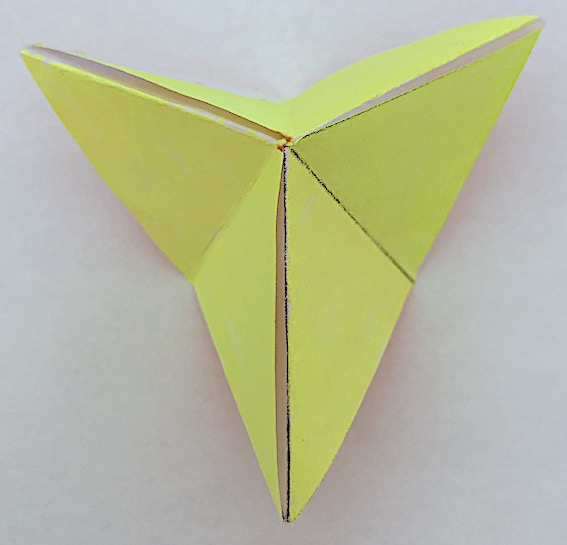
\includegraphics[height=3cm]{flexagone1} 
                  \qquad
                  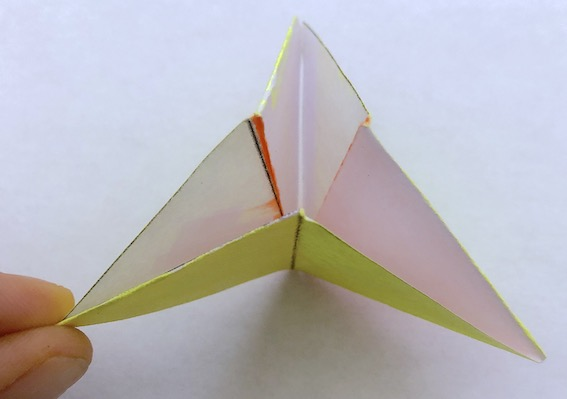
\includegraphics[height=3cm]{flexagone2} 
               \end{center}
            \item En réitérant le pliage, on obtient successivement les trois faces, une à une.
         \end{enumerate}
   
      \ARpartie{Pour aller plus loin}
         \begin{itemize}
            \item Un article, paru dan le magasine \og Pour la science \fg{} et écrit par {\it Jean-Paul Delahaye}, explique que l'on peut faire des flexagones avec autant de faces que l'on souhaite : \href{https://www.cristal.univ-lille.fr/~jdelahay/pls/2005/131.pdf}{\og Flexagones \fg}
            \item Il existe également des sites spécialisés, comme \href{http://www.flexagon.net}{Flexagone.net} qui propose de multiples modèles décorés à imprimer 
         \end{itemize}

\end{Maquette}